\documentclass{article}
\usepackage{amsmath} 
\usepackage{graphicx} 
\usepackage{authblk}
\usepackage{url}
\usepackage{hyperref}
\usepackage{multirow}
\usepackage{amssymb}
\usepackage{subcaption}
\usepackage[linesnumbered,boxed]{algorithm2e}

\topmargin 0.0cm
\oddsidemargin 0.2cm
\textwidth 16cm 
\textheight 21cm
\footskip 1.0cm

\title{Monte Carlo simulation of Two-dimensional Ising model}
\author[1]{Tong Li}
\affil[1]{Department of Physics and Astronomy, Michigan State University}
\date{}

\begin{document}
\maketitle
\begin{abstract}\label{abstract}
Ising model is a simple but important model to explain ferromagnetism. 
However, only one- and two-dimensional cases have been solved analytically. 
Therefore, it is necessary to develop a numerical method for the simulation of Ising model. 
In this work we focus on the application of Metropolis algorithm to the solve two-dimensional (2D) Ising model. 
We benchmark our numerical results with the analytical solution, 
and confirm that the system has a proper probability distribution and converges quickly to equilibrium in our simulation. 
The behaviors of phase transition around critical temperature also agree well with the analytical solution, 
and the critical temperature of infinitely large lattice is estimated to be 2.265 from our simulation, 
which is quite close to the theoretical value 2.269. 
Our work shows the success of Metropolis algorithm in the simulation of Ising model and 
we can simply extend it to higher dimensions.  

\end{abstract}

\section{Introduction}\label{intro} 
Ising model is a simple but important model for the explanation of magnetization. 
It assumes that atomic spins are located on a $N$-dimensional lattice grid, 
and these spins only have two discrete states, up ($\sigma=1$) or down ($\sigma=-1$). 
Only neighboring spins can interact with each other, and thus its Hamiltonian can be written as 
\begin{equation}\label{eq:hamiltonian}
H=-J\sum_{<kl>}^{N}\sigma_k\sigma_l\,,
\end{equation}
where $J>0$ and $<kl>$ indicates that we only sum over nearest neighbors. 
\par
In statistical physics, the equilibrium of a system described by Eq. \ref{eq:hamiltonian} should be solved using canonical ensemble, 
which involves a summation over all possible microscopic states to obtain the partition function. 
For $N$-dimensional Ising model with size $L$ in each dimension, 
the total number of all microscopic states is $2^{L^N}$, which cannot be simply summed over. 
The one- and two-dimensional cases has been solved analytically and they show several interesting properties of phase transition. 
But the exact solution of higher-dimensional Ising model is still unavailable, 
and thus numerical methods which avoid the summation over all possible states are required for the simulation of Ising model. 
\par
In this report, we discuss the Monte Carlo method for the simulation of two-dimensional (2D) Ising model 
and compare our results with the analytical solution. 
In Sec. \ref{theory} several properties shown in the analytical solution are discussed, for the comparison in Sec. \ref{results}. 
Sec. \ref{method} gives the outline of Monte Carlo algorithm we utilize for 2D Ising model, 
and then Sec. \ref{results} discusses the results of our simulation. 
Conclusions are given in Sec. \ref{conclude}. 

	
\section{Properties of 2D Ising model from its analytical solution}\label{theory}
In this section we discuss the properties of $L \times L$ Ising model with periodic boundary condition, 
which indicates that a spin on one boundary will interact with another spin on the opposite boundary. 
In other words, the summation over $<kl>$ in Eq. \ref{eq:hamiltonian} includes the following cases: 
\begin{equation}
k=(1,x),\ l=(L,x);\ k=(x,1),\ l=(x,L)
\end{equation}
where $(x,y)$ gives the coordinate of a spin in the $L \times L$ lattice. 

\subsection{The solution of $2 \times 2$ Ising model}\label{sec:2times2}
\begin{table}[tb]
	\centering
	\caption{All possible microscopic states of $2 \times 2$ Ising model. The energy is in the unit of $J$. }
	\begin{tabular}{cccc}
		\hline
		\hline 
		Number of spins up & Degeneracy & Energy & Magnetization \\ 
		\hline
		4 & 1 & -8 & 4 \\  
		3 & 4 & 0 & 2 \\ 
		2 & 4 & 0 & 0 \\ 
		2 & 2 & 8 & 0 \\ 
		1 & 4 & 0 & -2 \\ 
		0 & 1 & -8 & -4 \\ 
		\hline 
		\hline
	\end{tabular}
	\label{tab:2times2} 
\end{table}
For simplicity, we begin our discussion of the analytical solution from the $2 \times 2$ case. 
Table \ref{tab:2times2} shows all the possible microscopic states of  $2 \times 2$ Ising model. 
The corresponding partition function can be obtained by summing over all these microscopic states $\alpha$ 
\begin{equation}
Z=\sum_{\alpha}e^{-\beta E_\alpha}=2e^{8\beta}+2e^{-8\beta}+12=4\cosh\left(8\beta\right)+12\,,
\end{equation}
where $\beta=1/T$ and $T$ is temperature in the unit of $J$ (Boltzmann constant $k_B$ is absorbed into $T$). 
\par
Thus, the mean energy of the system (in the unit of $J$) is 
\begin{equation}
\langle E\rangle=-\frac{\partial \ln Z}{\partial \beta}=-\frac{8\sinh\left(8\beta\right)}{\cosh\left(8\beta\right)+3}\,. 
\end{equation}
The mean magnetization of the system is 
\begin{equation}
\langle|M|\rangle=\frac{1}{Z}\sum_{\alpha} |M_\alpha| e^{-\beta E_\alpha}=\frac{1}{Z}\left(8e^{8\beta}+4\right)
=\frac{2e^{8\beta}+1}{\cosh\left(8\beta\right)+3}\,. 
\end{equation}
The heat capacity is 
\begin{equation}\label{eq:cv}
C_V=\frac{\partial \langle E\rangle}{\partial T}=-\beta^2\frac{\partial \langle E\rangle}{\partial \beta}
=\beta^2\frac{64\left[1+\cosh\left(8\beta\right)\right]}{\left[6+\cosh\left(8\beta\right)\right]^2}
=\beta^2\left(\langle E^2\rangle-\langle E\rangle^2\right)\,,
\end{equation}
where 
\begin{equation}
\langle E^2\rangle=\frac{1}{Z}\sum_{\alpha}E^2_\alpha e^{-\beta E_\alpha}=\frac{64\cosh\left(8\beta\right)}{\cosh\left(8\beta\right)+3}\,. 
\end{equation}
Similarly, we have 
\begin{equation}
\langle M^2\rangle=\frac{1}{Z}\sum_{\alpha} M^2_\alpha e^{-\beta E_\alpha}=\frac{8\left(e^{8\beta}+1\right)}{\cosh\left(8\beta\right)+3}\,, 
\end{equation}
and define susceptibility as 
\begin{equation}\label{eq:chi}
\chi=\beta\left(\langle M^2\rangle -\langle |M|\rangle ^2\right)\,. 
\end{equation}
Above results can be used to benchmark the Monte Carlo algorithm developed for 2D Ising model. 

\subsection{Properties of phase transition in 2D Ising model}\label{sec:transition}
One important aspect of the analytical solution of 2D Ising model is the second-order phase transition 
at a nonzero critical temperature $T_C$. 
There is a sharp transition from nonzero $\langle|M|\rangle $ to $\langle|M|\rangle=0$ 
when temperature $T$ increases from $T<T_C$ to $T>T_C$. 
In this section we do not discuss the details of the analytical solution of 2D Ising model. 
Instead, we will show several important properties of phase transition in 2D Ising model, 
which are used to benchmark our simulation. 
\par
Near $T_C$ we can characterize the behavior of many physical quantities by a power law.
For 2D Ising model, the mean magnetization is given by
\begin{equation}
\langle M(T) \rangle \sim \left(T-T_C\right)^{\beta}\,,
\end{equation}
where $\beta=1/8$ is a critical exponent. A similar relation applies to heat capacity 
\begin{equation}
C_V(T) \sim \left|T_C-T\right|^{\alpha}\,,
\end{equation}
and the susceptibility
\begin{equation}
\chi(T) \sim \left|T_C-T\right|^{\gamma}\,,
\end{equation}
with $\alpha = 0$ and $\gamma = 7/4$. 
It should be noted that $\alpha=0$ does not mean that $C_V$ is continuous around $T_C$. 
The analytical solution shows that $C_V$ will logarithmically diverge at $T_C$. 
Another important quantity is called correlation length, which is expected
to be of the order of the lattice spacing for $T>> T_C$. Because the spins
become more and more correlated as $T$ approaches $T_C$, the correlation
length increases as we get closer to the critical temperature. The divergent
behavior of $\xi$ near $T_C$ is 
\begin{equation}
\xi(T) \sim \left|T_C-T\right|^{-\nu}\,,
\label{eq:xi}
\end{equation}
with $\nu=1$. 
A second-order phase transition is characterized by a
correlation length which spans the whole system.
Since we are always limited to a finite lattice, $\xi$ will
be proportional with the size of the lattice. 
Through so-called finite size scaling relations
it is possible to relate the behavior at finite lattices with the 
results for an infinitely large lattice.
The critical temperature scales then as
\begin{equation}
T_C(L)-T_C(L=\infty) = aL^{-1/\nu}\,,
\label{eq:tc}
\end{equation}
where $a$ is a constant and $\nu$ is defined in Eq. \ref{eq:xi}. 
We set $T=T_C$ and obtain a mean magnetization
\begin{equation}
\langle M(T) \rangle \sim \left(T-T_C\right)^{\beta}
\rightarrow L^{-\beta/\nu}\,,
\label{eq:scale1}
\end{equation}
heat capacity
\begin{equation}
C_V(T) \sim \left|T_C-T\right|^{-\gamma} \rightarrow L^{\alpha/\nu},
\label{eq:scale2}
\end{equation}
and susceptibility
\begin{equation}
\chi(T) \sim \left|T_C-T\right|^{-\alpha} \rightarrow L^{\gamma/\nu}\,.
\label{eq:scale3}
\end{equation}
\par
The exact solution gives $\nu=1$ and $T_C=\frac{2}{\ln\left(1+\sqrt{2}\right)}\approx 2.269$ 
(in the unit of $J$) when $L\rightarrow\infty$. 
With the help of Eq. \ref{eq:tc}, we can use our simulation results of different $L$ to extract $T_C$ for $L\rightarrow\infty$, 
which will be done in Sec. \ref{results}. 

	
\section{Monte Carlo methods for Ising model}\label{method}
In our work the Metropolis algorithm is adopted for the simulation of Ising model. 
This algorithm is based on the theory of Markov chain and detailed balance. 
In the example of Ising model, the transition rate between two microscopic states $i$ and $j$ should satisfy 
\begin{equation}\label{eq:Wfrac}
\frac{W(j \rightarrow i)}{W(i \rightarrow j)}=\frac{w_i}{w_j}=e^{-\beta\left(E_i-E_j\right)}\,,
\end{equation}
with $w_i=\frac{1}{Z}e^{-\beta E_i}$ 
to obtain an equilibrated (and detailed-balanced) probability distribution given by canonical ensemble. 
We can model $W(j \rightarrow i)$ as a product of the probability $T(j \rightarrow i)$ to make a transition from $j$ to $i$ 
and the probability $A(j \rightarrow i)$ to accept this transition, namely 
\begin{equation}
W(j \rightarrow i)=T(j \rightarrow i)A(j \rightarrow i)\,.
\end{equation}
In the simulation of Ising model, we have no physical insight of $T(j \rightarrow i)$, 
so we can simply assume that all $T(j \rightarrow i)$ are the same. 
Then Eq. \ref{eq:Wfrac} can be rewritten as 
\begin{equation}\label{eq:Afrac}
\frac{A(j \rightarrow i)}{A(i \rightarrow j)}=e^{-\beta\left(E_i-E_j\right)}\,,
\end{equation}
which describes the probability of accepting a transition from $j$ to $i$ in our simulation. 
\par
\begin{algorithm}[tb]
	\caption{Metropolis algorithm for the simulation of Ising model. }
	\label{alg::metropolis}
	\KwIn{Size of the system $L$, temperature $T$, number of Monte Carlo cycles $MC$. }
	\KwOut{$\langle E \rangle$, $\langle E^2 \rangle$, $\langle |M| \rangle$, $\langle M^2 \rangle$, $C_V$ and $\chi$. } 
	Initialize spin lattice $a$ (in an ordered or random way)\;
	Calculate $E$, $E^2$, $|M|$, $M^2$ of the initial lattice\; 
	$E_{tot}=0,\,E^2_{tot}=0,\,|M|_{tot}=0,\,M^2_{tot}=0$\;
	\For{$i=1;i<=MC;i++$}
	{
		\For{$j=1;j<=L;j++$}
		{
			\For{$k=1;k<=L;k++$}
			{
				$r=$ a uniformly distributed random number in $[0,1]$\;
				Flip spin at position $(j,k)$\;
				Calculate the change of energy $\Delta E$\; 
				\If{$\Delta E < 0\ \mathrm{or}\ r<\exp\left(-\Delta E/T\right)$}
				{
					Accept this spin flip\; 
					Update $E$, $E^2$, $|M|$, $M^2$\;
				}
				\Else
				{
					Reverse this spin flip\;
				}
			Add $E$, $E^2$, $|M|$, $M^2$ to their corresponding ``tot" variables\; 
			}
		}
	}
	Calculate the average $\langle E \rangle$, $\langle E^2 \rangle$, $\langle |M| \rangle$, $\langle M^2 \rangle$ by dividing $L^2MC$\; 
	Calculate $C_V$ and $\chi$ by Eq. \ref{eq:cv} and \ref{eq:chi}\;
\end{algorithm}
Based on Eq. \ref{eq:Afrac} we can develop a simulation algorithm shown in Algorithm \ref{alg::metropolis}. 
The main idea is that we flip one spin every time and use a random number $r$, which distributes uniformly in $[0,1]$, to determine whether to accept this flip based on Eq. \ref{eq:Afrac}. 
If this flip reduces the energy or $r<\exp\left(-\Delta E/T\right)$ ($\Delta E$ is the energy change in the transition) we will accept. 
In one Monte Carlo cycle we iterate through the full lattice and try to flip each spin. 
Physical quantities $\langle E \rangle$, $\langle E^2 \rangle$, $\langle |M| \rangle$, $\langle M^2 \rangle$ 
are obtained by averaging them in the Monte Carlo process. 

	
\section{Results and discussion}\label{results}
In this section we will discuss the results given by our Monte Carlo simulation of 2D Ising model. 
Sec. \ref{sec:2times2result} gives the results of $2 \times 2$ case for benchmark. 
In Sec. \ref{sec:detailresult} we discuss the change of energy and magnetization in the Monte Carlo process for $20\times20$ lattice 
and show their probability distributions. 
In Sec. \ref{sec:transitionresult} the phenomenon of phase transition in 2D Ising model is discussed for different lattice size. 

\subsection{Benchmark: $2 \times 2$ case}\label{sec:2times2result}
\begin{table}[tb]
	\centering
	\caption{Results for $2\times2$ case with temperature $T=1.0$. Analytical results are provided for benchmark. 
	Energy is in the unit of $J$. }
	\begin{tabular}{cccccc}
		\hline
		\hline
		Number of Monte Carlo cycles $MC$ & 10 & 100 & 1000 & 10000 & Analytical \\ 
		\hline
		Mean energy $\langle E \rangle$ & -7.2 & -7.92 & -7.986 & -7.988 & -7.98393\\ 
		Mean magnetization $\langle |M| \rangle$ & 3.75 & 3.975 & 3.9955 & 3.99625 & 3.99263\\ 
		Mean square of energy $\langle E^2 \rangle$ & 57.6  & 63.36 & 63.888 & 63.904 & 63.8714\\ 
		Mean square of magnetization $\langle M^2 \rangle$ & 14.7 & 15.87 & 15.977 & 15.9805 & 15.9732\\ 
		Heat capacity $C_V$ & 5.76 & 0.6336 & 0.111804 & 0.095856 & 0.128329\\ 
		Susceptibility $\chi$ & 0.6375 & 0.069375 & 0.0129798 & 0.0104859 & 0.0320873\\ 
		\hline
		\hline 
	\end{tabular} 
	\label{tab:2times2result}
\end{table}
Table \ref{tab:2times2result} gives the quantities we obtain from our Monte Carlo simulation of $2\times2$ lattice with temperature $T=1.0$. 
As the number of Monte Carlo cycles $MC$ increases, our results get closer to the analytical values. 
For $MC=1000$ our results are close enough to the analytical values for benchmark purpose. 
However, we can notice that both heat capacity $C_V$ and susceptibility $\chi$ do not agree well with the analytical results, 
and they have some fluctuations as $MC$ increases. 
The reason is that both $\langle E^2 \rangle$ and $\langle E \rangle^2$ are large but close to each other, 
so their difference, which determines $C_V$, will have a large numerical error. 
This is unavoidable when $C_V$ and $\chi$ are small. 

\subsection{Convergence and probability distribution}\label{sec:detailresult}
\begin{figure}[tb]
	\begin{subfigure}[tb]{0.5\textwidth}
		\centering
		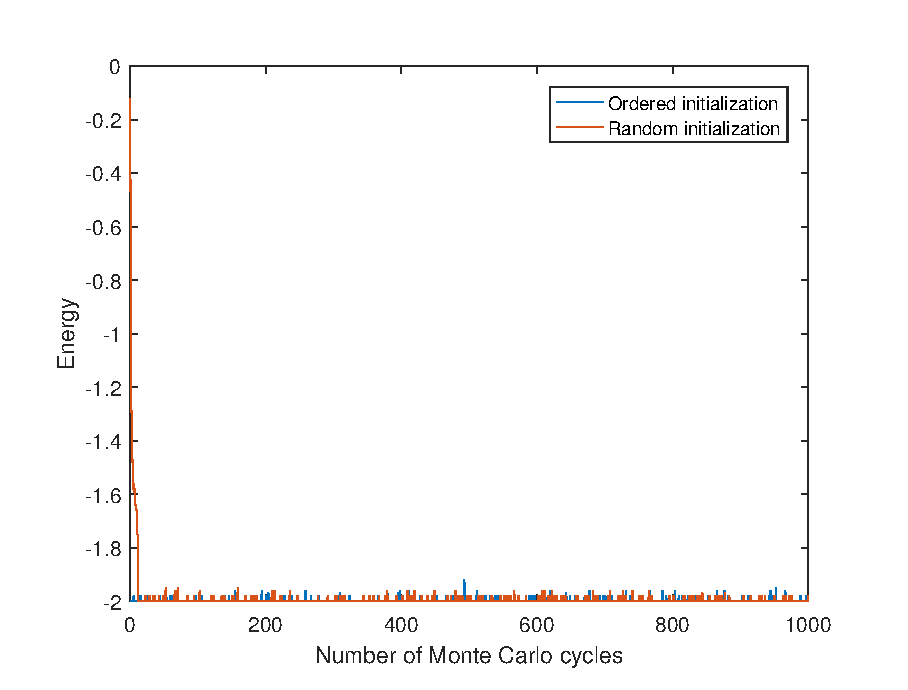
\includegraphics[width=0.7\textwidth]{Process_ene_lowT.eps}
		\caption{$T=1.0$}
	\end{subfigure}
	~
	\begin{subfigure}[tb]{0.5\textwidth}
		\centering
		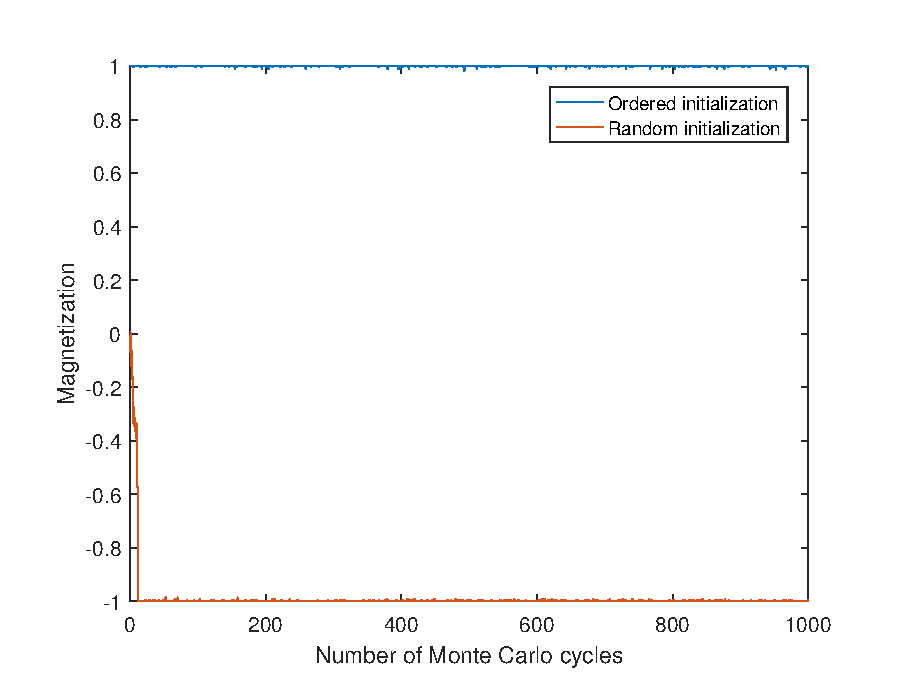
\includegraphics[width=0.7\textwidth]{Process_mag_lowT.eps}		
		\caption{$T=1.0$}
	\end{subfigure}
	~
	\begin{subfigure}[tb]{0.5\textwidth}
		\centering
		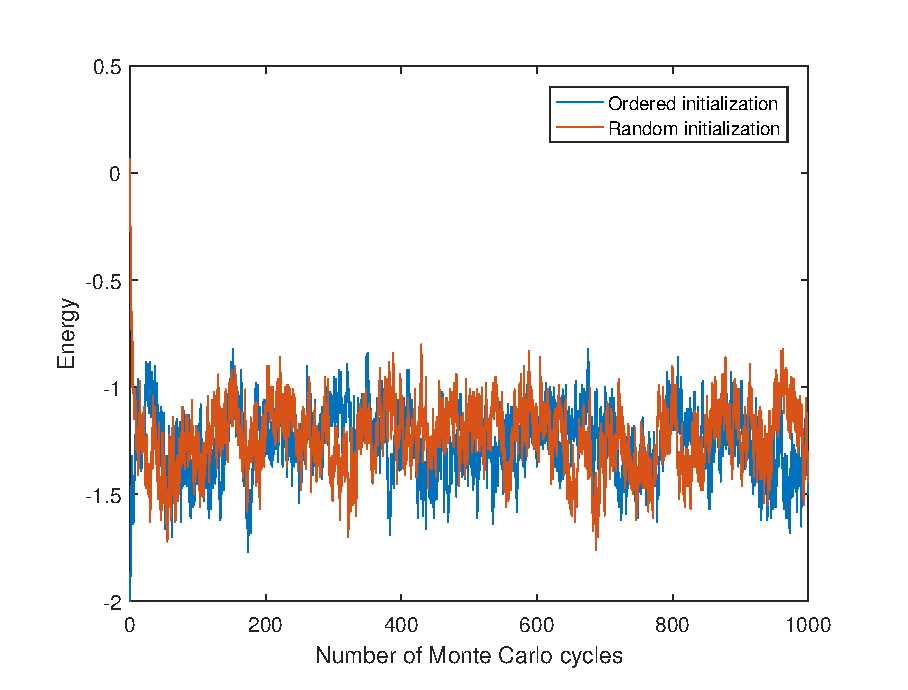
\includegraphics[width=0.7\textwidth]{Process_ene_highT.eps}		
		\caption{$T=2.4$}
	\end{subfigure}
	~
	\begin{subfigure}[tb]{0.5\textwidth}
		\centering
		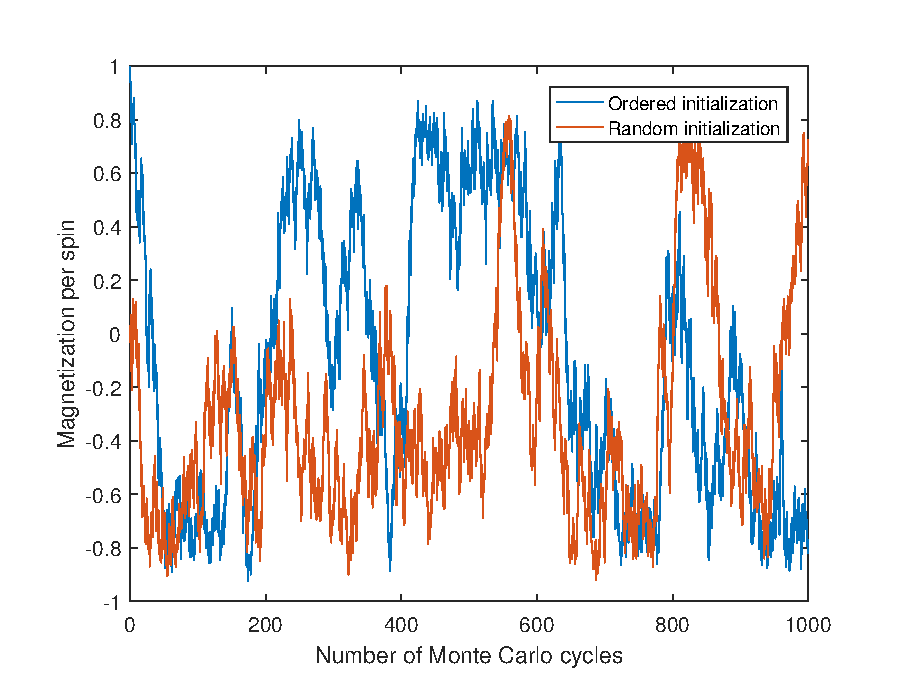
\includegraphics[width=0.7\textwidth]{Process_mag_highT.eps}		
		\caption{$T=2.4$}
	\end{subfigure}
	\caption{Energy and magnetization per spin as a function of the number of Monte Carlo cycles. 
	Energy is in the unit of $J$. Temperature $T=1.0$ or $2.4$. }
	\label{fig:process}
\end{figure}
For our simulation, it is important to know when the system become equilibrated, 
which determines how many Monte Carlo cycles are necessary. 
Fig. \ref{fig:process} shows the change of energy and magnetization as a function of the number of Monte Carlo cycles $MC$ 
for $20 \times 20$ lattice with temperature $T=1.0$ and $T=2.4$. 
Blue lines are the results of ordered initialization (starting from all spins pointing up) 
and orange lines are the results of random initialization (starting from random spin orientation). 
From Fig. \ref{fig:process}, we can see that the energy of the system converges quite fast, 
and different initializations give the same results after some Monte Carlo cycles. 
For $T=1.0$, the system soon goes to an ordered phase with very small fluctuations. 
For $T=2.4$, higher temperature will raise the probability of the system being at excitation states. 
Thus, the energy has a larger fluctuation around its mean value, 
and the magnetization also oscillates dramatically 
because states with different magnetization can have the same energy (degeneracy). 
\par
\begin{figure}[tb]
	\begin{subfigure}[tb]{0.5\textwidth}
		\centering
		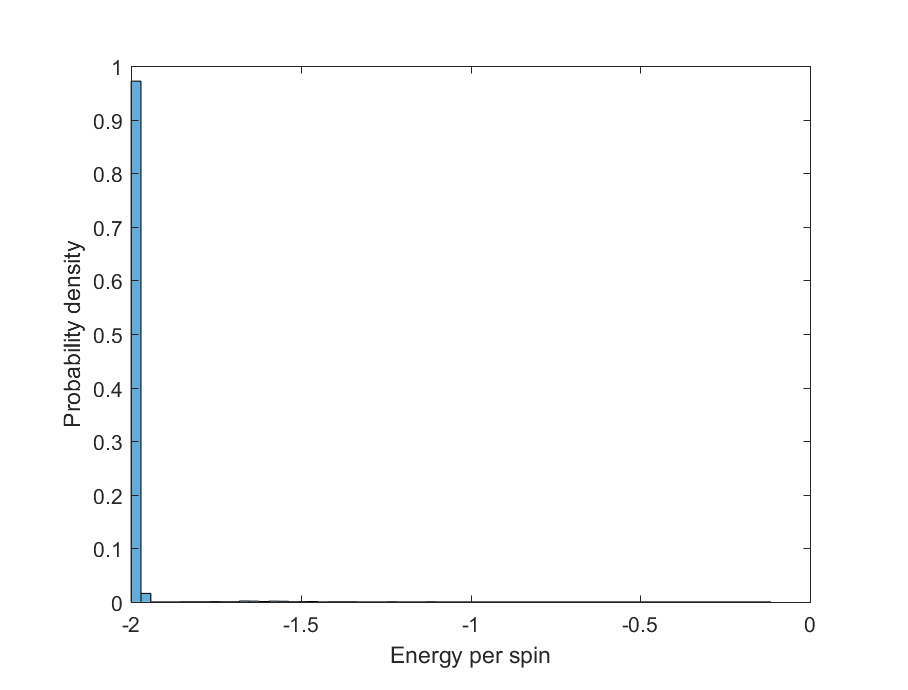
\includegraphics[width=0.7\textwidth]{Prob_ene_lowT.eps}
		\caption{$T=1.0$}
	\end{subfigure}
	~
	\begin{subfigure}[tb]{0.5\textwidth}
		\centering
		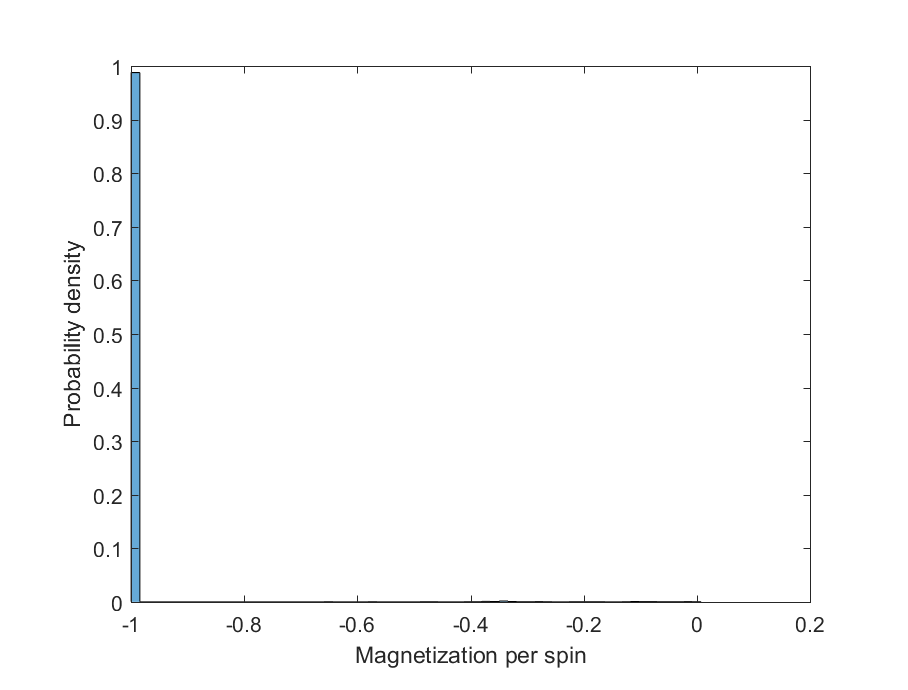
\includegraphics[width=0.7\textwidth]{Prob_mag_lowT.eps}		
		\caption{$T=1.0$}
	\end{subfigure}
	~
	\begin{subfigure}[tb]{0.5\textwidth}
		\centering
		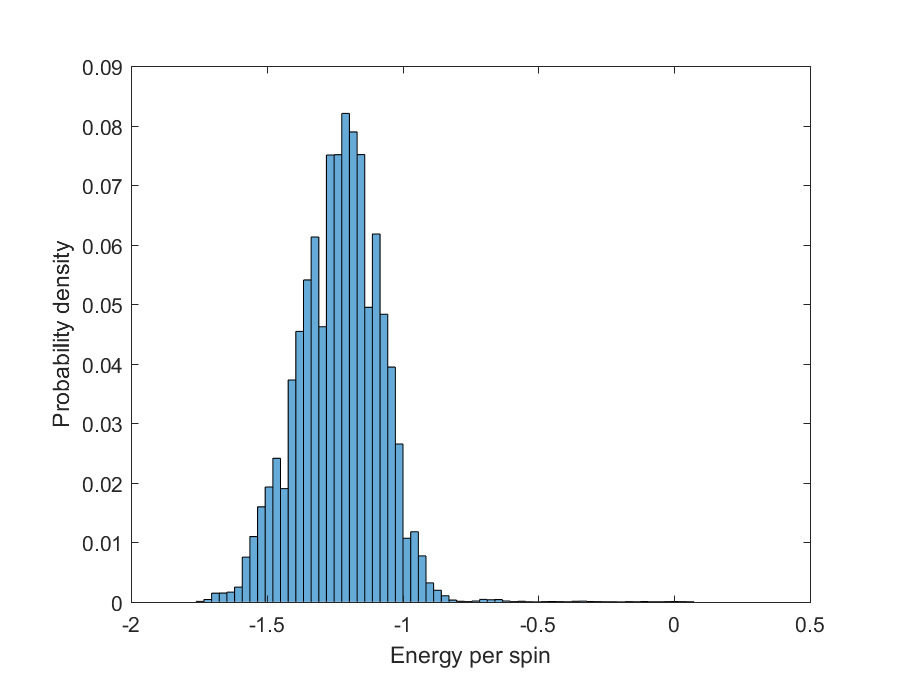
\includegraphics[width=0.7\textwidth]{Prob_ene_highT.eps}		
		\caption{$T=2.4$}
	\end{subfigure}
	~
	\begin{subfigure}[tb]{0.5\textwidth}
		\centering
		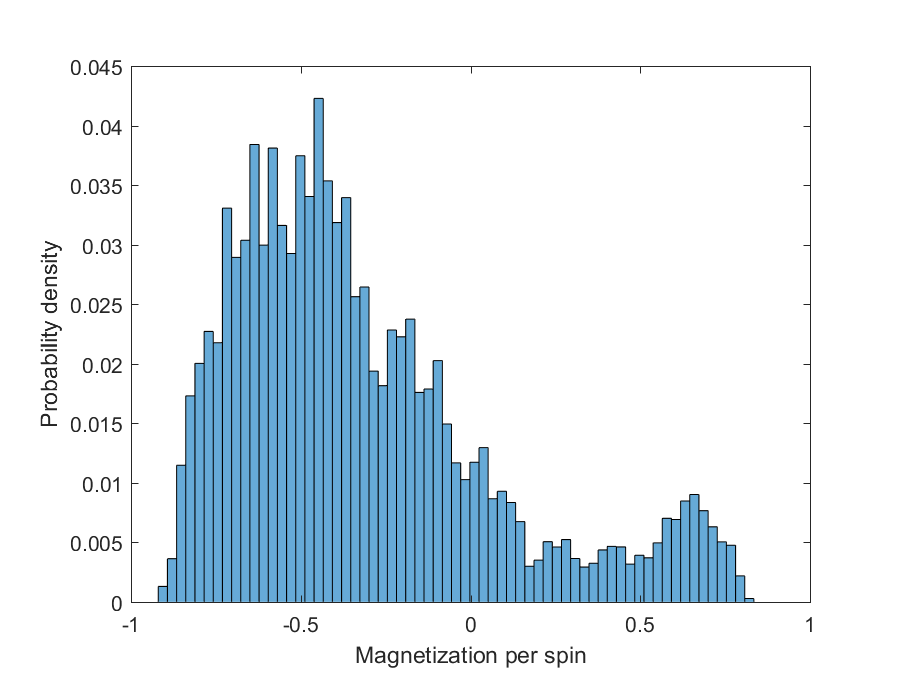
\includegraphics[width=0.7\textwidth]{Prob_mag_highT.eps}		
		\caption{$T=2.4$}
	\end{subfigure}
	\caption{Probability distribution of energy and magnetization per spin. 
		Energy is in the unit of $J$. Temperature $T=1.0$ or $2.4$. }
	\label{fig:prob}
\end{figure}
Fig. \ref{fig:prob} gives the distributions of energy and magnetization per spin in the Monte Carlo process with random initialization. 
For $T=1.0$, the system is almost always stays at an ordered phases, 
and thus we have a high peak of magnetization per spin at $M/L^2=1$, and a high peak of energy per spin at $E/L^2=-2$. 
For $T=2.4$, the distribution of energy centers at the most probable value, which is approximately the mean value; 
the distribution of magnetization is broader because of states with different magnetization but the same energy. 

\subsection{Phase transition}\label{sec:transitionresult}
\begin{figure}[tb]
	\begin{subfigure}[tb]{0.5\textwidth}
		\centering
		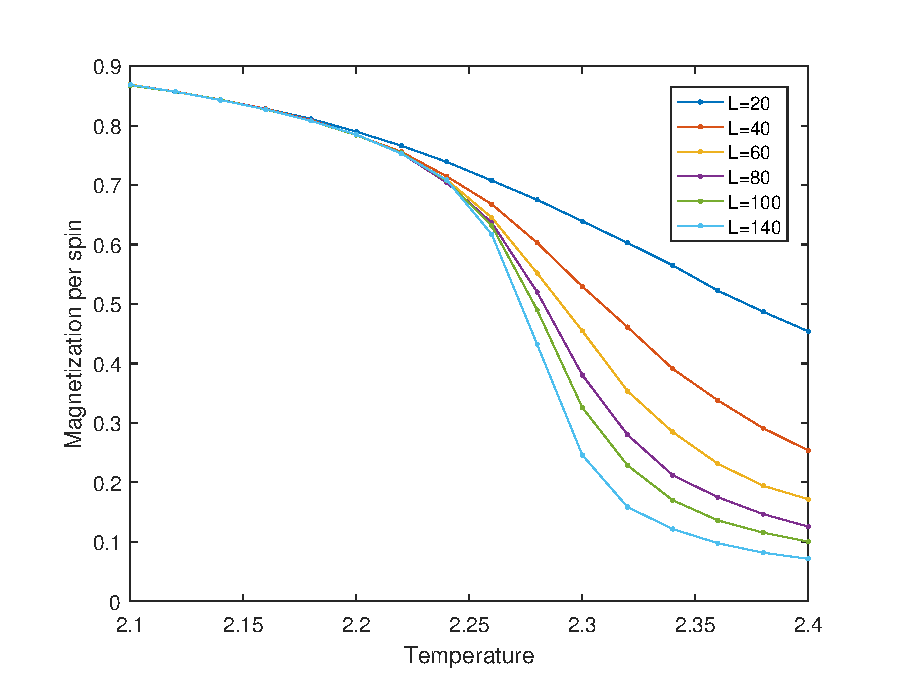
\includegraphics[width=0.7\textwidth]{Tran_mag.eps}
		\caption{}
	\end{subfigure}
	~
	\begin{subfigure}[tb]{0.5\textwidth}
		\centering
		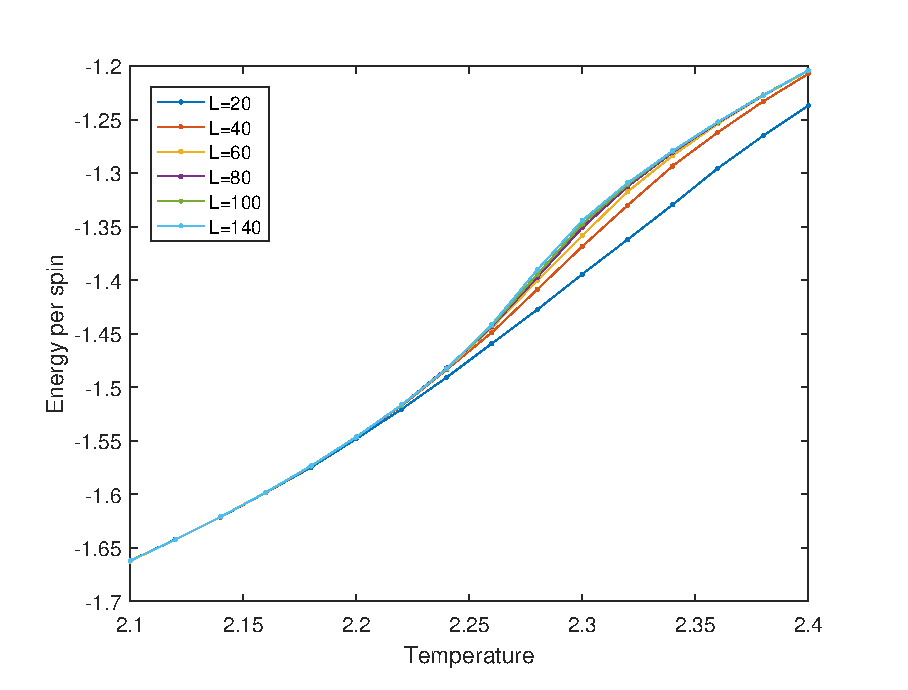
\includegraphics[width=0.7\textwidth]{Tran_ene.eps}		
		\caption{}
	\end{subfigure}
	~
	\begin{subfigure}[tb]{0.5\textwidth}
		\centering
		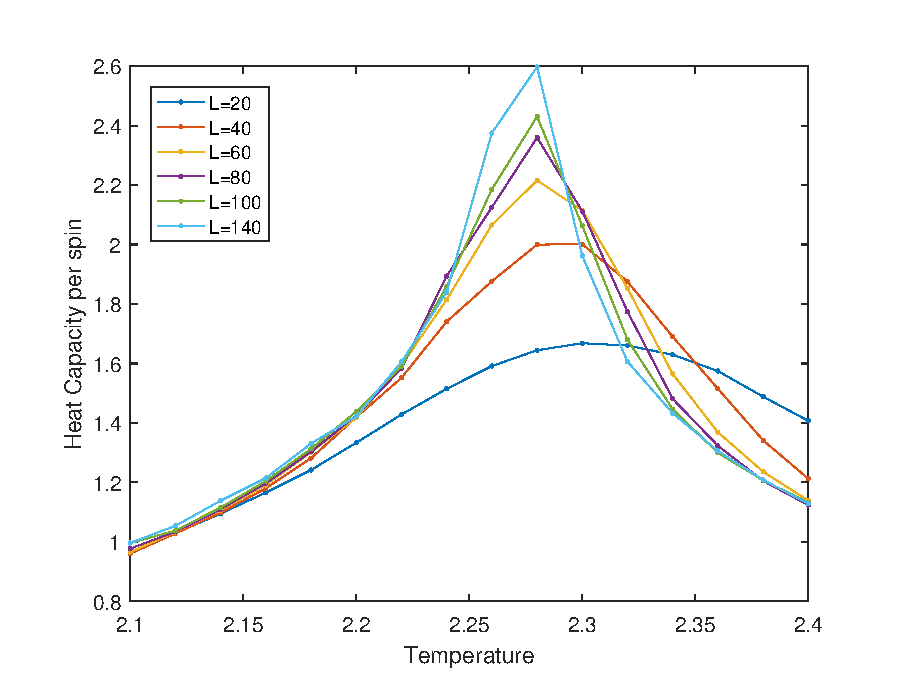
\includegraphics[width=0.7\textwidth]{Tran_Cv.eps}		
		\caption{}
	\end{subfigure}
	~
	\begin{subfigure}[tb]{0.5\textwidth}
		\centering
		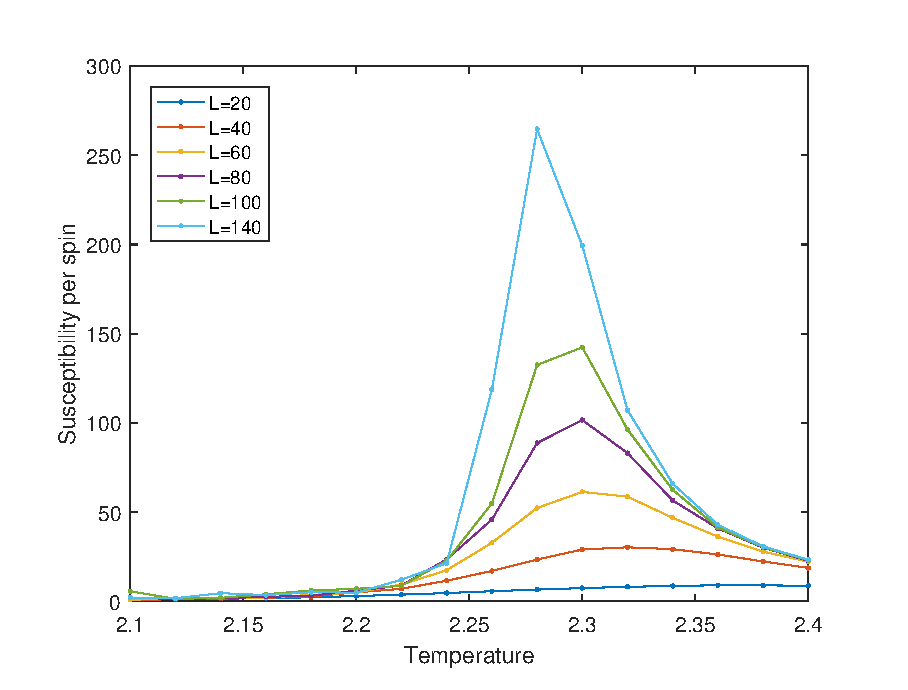
\includegraphics[width=0.7\textwidth]{Tran_sus.eps}		
		\caption{}
		\label{fig:transition_sus}
	\end{subfigure}
	\caption{Energy, magnetization, heat capacity and susceptibility per spin as a function of temperature
	with different lattice size $L=20,\,40,\,60,\,80,\,100,\,140$ in the temperature range $T\in[2.1,2.4]$. 
	Temperature step is 0.02. }
	\label{fig:transition}
\end{figure}
To investigate the phase transition in Ising model, we perform calculations with different lattice size 
$L=20,\,40,\,60,\,80,\,100,\,140$ in the temperature range $T\in[2.1,2.4]$. 
Temperature step is 0.02 and the number of Monte Carlo cycles is $10^6$. 
Fig. \ref{fig:transition} gives the energy, magnetization, heat capacity and susceptibility per spin as a function of temperature. 
It can be seen that around $T=2.28$ the magnetization drops fast as $T$ increases, 
indicating that the system undergoes a transition from an ordered phase to a disordered phase. 
This transition is not dramatic when $L$ is small (e.g. $L=20$ and $40$), which results from the finite size of the system. 
The energy of the system, however, changes smoothly when the phase transition occurs, 
which is a characteristic of a second-order transition. 
Both heat capacity and susceptibility have a high peak around the transition temperature, 
which agrees with the divergence of these two quantities shown in the analytical solution. 
\par
By Eq. \ref{eq:tc} we can estimate $T_C$ for an infinitely large system from the results with finite $L$. 
It is quite difficult to determine the critical temperature from Fig. \ref{fig:transition} 
because our resolution is not small enough and the peaks of $C_V$ and $\chi$ do not coincide. 
From the peaks of $\chi$ (Fig. \ref{fig:transition_sus}) we estimate that $T_C(L=60)=2.3$ and $T_C(L=140)=2.28$. 
By Eq. \ref{eq:tc} and $\nu=1$ we obtain 
\begin{equation}
\left\{
\begin{array}{c}
a=2.1\,,  \\
T_C(L=\infty)=2.265\,.  \\
\end{array}
\right.
\end{equation}
Our estimation is close to the analytical result 2.269. 
	
\section{Conclusion}\label{conclude}
In this work, we investigate two methods, Euler's forward and Velocity-Verlet method, 
to solve a set of first-order ordinary differential equations with initial conditions. 
To test the performance of these algorithms, 
we use them to calculate the evolution of the Earth-Sun, Earth-Sun-Jupiter and whole solar system. 
Our comparison shows that the Verlet method can better describe the characteristics of motion in these systems than Euler's method. 
We conclude that Verlet method is more stable and thus better to use. 
We also use Verlet method to calculate the perihelion precession of Mercury by adding a relativistic correction to the gravitational force 
and obtain a $43''$ per century precession which is the same as the analytical solution. 
	
\section*{Acknowledgments}
We are grateful for the sincere guidance from Prof. Morten Hjorth-Jensen. 
	
\nocite{*} 
\bibliographystyle{unsrt}
\bibliography{proj4_ref}
\end{document}